\documentclass[a4paper,12pt]{article}

\usepackage[utf8]{inputenc} % allow utf-8 input
\usepackage{hyperref}       % hyperlinks
\usepackage{url}            % simple URL typesetting
\usepackage{booktabs}       % professional-quality tables
\usepackage{amsfonts}       % blackboard math symbols
\usepackage{nicefrac}       % compact symbols for 1/2, etc.
\usepackage{microtype}      % microtypography
\usepackage{graphicx}       % include graphics
\usepackage{subcaption}     % subfigures
\usepackage{float}          % placement of floats
\usepackage{fancyhdr}       % head notes and foot notes
\usepackage{bbm}            % Nice symbols
\usepackage{mathtools}      % Math tools like operators
\usepackage{listings}       % Write code in a listing
\usepackage[left=2.5cm,right=2.5cm,top=3cm,bottom=3cm]{geometry}

\graphicspath{ {assets/} }

% Operators
\DeclarePairedDelimiter\abs{\lvert}{\rvert} % abs
\DeclarePairedDelimiter\norm{\lVert}{\rVert} % norm
\DeclareMathOperator*{\argmax}{arg\,max} % argmax
\newcommand{\p}{\mathbbm{P}} % Big P for probabilties
\newcommand{\pd}[2]{\frac{\partial #1}{\partial #2}}  % Partial derivative

% To prevent the tilde from being printing above with lstlisting
\lstset{
    literate={~} {$\sim$}{1},
    showstringspaces=false,
    numbers=left,
    breaklines=true
}

% Sections naming conventions
\renewcommand{\thesection}{\arabic{section}}
\renewcommand{\thesubsection}{(\alph{subsection})}
\renewcommand{\thesubsubsection}{\roman{subsubsection}.}

% Head and foot notes
\pagestyle{fancy}
\fancyhf{}
\lhead{Louis MARTIN}
\rhead{Big Data Processing and Analytics: Assignment 1}
\rfoot{Page \thepage}

\begin{document}

\title{Big Data Processing and Analytics: Assignment 1}
\author{Louis MARTIN\\
\href{mailto:louis.martin@student.ecp.fr}{\tt louis.martin@student.ecp.fr}}

\maketitle

In this assignment we are going to create an inverted index on a corpus
including the complete works of William Shakespear, Mark Twain and Jane Austen
using Hadoop's MapReduce framework.

\section{Setup}
\subsection{System specifications}

\begin{itemize}
    \item \textbf{Operating system}:\\
    Ubuntu 16.04 (Native)
    \item \textbf{System specifictations}:\\
    Model: Dell Inspiron 17R 5720\\
    Processor: i5-3210M\\
    Cores: 2\\
    Threads: 4\\
    Ram: 8 GB\\
    Storage: 256GB SSD (MLC)
    \item \textbf{Java version}:\\
    openjdk version "1.8.0\_121"\\
    OpenJDK Runtime Environment (build 1.8.0\_121-8u121-b13-0ubuntu1.16.04.2-b13)\\
    OpenJDK 64-Bit Server VM (build 25.121-b13, mixed mode)
    \item \textbf{Haddop version}:\\
    Hadoop 2.7.3\\
    Subversion https://git-wip-us.apache.org/repos/asf/hadoop.git -r baa91f7c6bc9cb92be5982de4719c1c8af91ccff\\
    Compiled by root on 2016-08-18T01:41Z\\
    Compiled with protoc 2.5.0\\
    From source with checksum 2e4ce5f957ea4db193bce3734ff29ff4\\
    This command was run using /usr/local/hadoop/share/hadoop/common/hadoop-common-2.7.3.jar\\

\end{itemize}

Hadoop was installed using \href{https://www.digitalocean.com/community/tutorials/how-to-install-hadoop-in-stand-alone-mode-on-ubuntu-16-04}{this tutorial} and configured using \href{https://hadoop.apache.org/docs/stable/hadoop-project-dist/hadoop-common/SingleCluster.html}{this tutorial}.


\subsection{Configuration}
The configuration comes from the \href{https://hadoop.apache.org/docs/stable/hadoop-project-dist/hadoop-common/SingleCluster.html}{official documentation} for a single Hadoop node cluster.
The following configuration files allows Hadoop and YARN to run in a pseudo-distributed mode.
\begin{itemize}
    \item \textbf{core-site.xml:}
    \lstinputlisting[firstline=19, lastline=24, language=xml]{assets/core-site.xml}
    \item \textbf{hdfs-site.xml:}
    \lstinputlisting[firstline=19, lastline=24, language=xml]{assets/hdfs-site.xml}
    \item \textbf{mapred-site.xml:}
    \lstinputlisting[firstline=19, lastline=24, language=xml]{assets/mapred-site.xml}
    \item \textbf{yarn-site.xml:}
    \lstinputlisting[firstline=15, lastline=29, language=xml]{assets/yarn-site.xml}
    \item \textbf{Commands to set up HDFS and YARN:}
    \begin{lstlisting}[language=bash]
      # Format the filesystem
      hdfs namenode -format
      # Start HDFS
      start-dfs.sh

      # Create directories to execute MapReduce jobs
      hdfs dfs -mkdir /user
      hdfs dfs -mkdir /user/louis

      # Put the data in HDFS
      hdfs dfs -put ~/dev/bdpa/a1/data data

      # Start YARN Ressource manager
      start-yarn.sh
    \end{lstlisting}
\end{itemize}


\subsection{Bugs encountered}
I encountered a bug while running the MapReduce jobs where I would be logged out and all my processes would be killed with no warning.
After investigation, I found that \href{https://bugs.launchpad.net/ubuntu/+source/procps/+bug/1610499}{this is a known bug referenced here} and caused by /bin/kill in ubuntu 16.04.

I compiled propcps-3.3.10 from source to solve the problem as indicated in launchpad but to no avail.
\begin{lstlisting}[language=bash]
  # (1) download the sourcecode
  sudo apt-get source procps

  # (2) install dependency
  sudo apt-get build-dep procps

  # (3) compile procps
  cd procps-3.3.10
  sudo dpkg-buildpackage
\end{lstlisting}


I tried another solution from \href{http://stackoverflow.com/questions/38419078/logouts-while-running-hadoop-under-ubuntu-16-04}{this stackoverflow thread} but it didn't work either.
The supposed fix was to add
\begin{lstlisting}
  [login]
  KillUserProcesses=no
\end{lstlisting}
to \lstinline{/etc/systemd/logind.conf} and restart.


\section{Inverted index}

In order to facilitate compiling the $.java$ files into $.jar$ files, I created
the $compile.sh$ script which takes as input parameter the name of the main class of the $.java$ file.
\\Example: \lstinline{./compile.sh StopWords}.
\\ \textbf{compile.sh}:
\lstinputlisting[language=bash]{assets/compile.sh}

\subsection{(30) Stop words}


Based on the wordcount example from the \href{https://hadoop.apache.org/docs/stable/hadoop-mapreduce-client/hadoop-mapreduce-client-core/MapReduceTutorial.html}{official documentation},
we implement a MapReduce program that retrieves all the stopwords from a corpus,
i.e it retrieves the words with wordcount greater than 4000.
\\The file is \textbf{StopWords.java}
\begin{itemize}
  \item \textbf{Mapper}:\\
  This mapper splits a string into words (tokens) and outputs one (key, value) pair
  for each word with the key being the word and the value equal to 1.
  \lstinputlisting[firstnumber=18, firstline=18, lastline=34, language=java]{assets/StopWords.java}
  \item \textbf{Reducer}:\\
  The reducers, simply counts the number of occurences of each key writes it to
  the output file only if its count is greater than 4000.
  \lstinputlisting[firstnumber=36, firstline=36, lastline=53, language=java]{assets/StopWords.java}
  \item \textbf{Job configuration}:\\
  The MapReduce task is set to write the output as a csv file.
  We can set the number of reducers, combiner and compression through command line
  arguments.
  \lstinputlisting[firstnumber=55, firstline=55, lastline=101, language=java]{assets/StopWords.java}
  \item \textbf{Script that runs the experiments}:\\
  We run the set of experiments with the \textbf{run\_stopwords.sh} script.
  This script executes the StopWords MapReduce task with different parameters
  and merges all the outputs into a csv file in HDFS.
  \lstinputlisting[language=bash]{assets/run_stopwords.sh}

\end{itemize}

\subsubsection{(10) 10 Reducers and no Combiner}
The running time with 10 reducers is \textbf{126 seconds}.
\begin{figure}[!htbp]
  \centering
  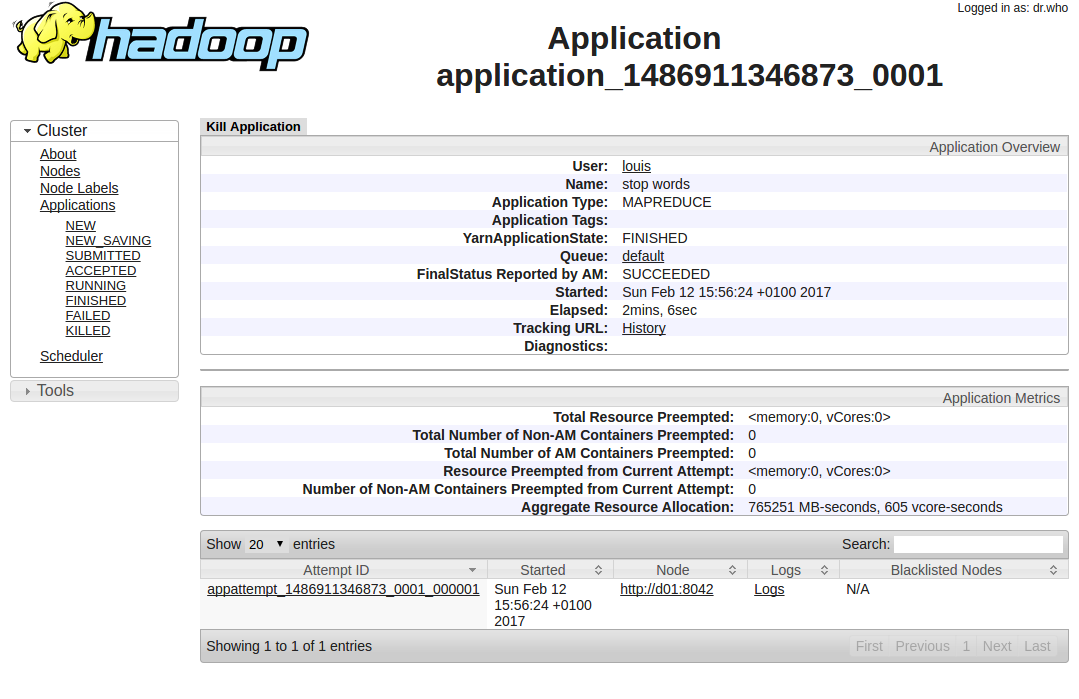
\includegraphics[width=.6\textwidth]{stopwords_10_reducers.png}
\end{figure}
\subsubsection{(10) 10 Reducers and Combiner}
The running time with 10 reducers and 1 combiner is \textbf{105 seconds}.
The running time is lower with the combiner. Indeed the combiner takes the output
of each mapper separately and tries to reduce as many (key, value) pairs coming
from this specific mapper as it can.
Combining the data like this will lower the load for the reducers, and all the
intermediary steps like for example sorting all the (key, value) pairs and assign them
to each reducer.
\begin{figure}[!htbp]
  \centering
  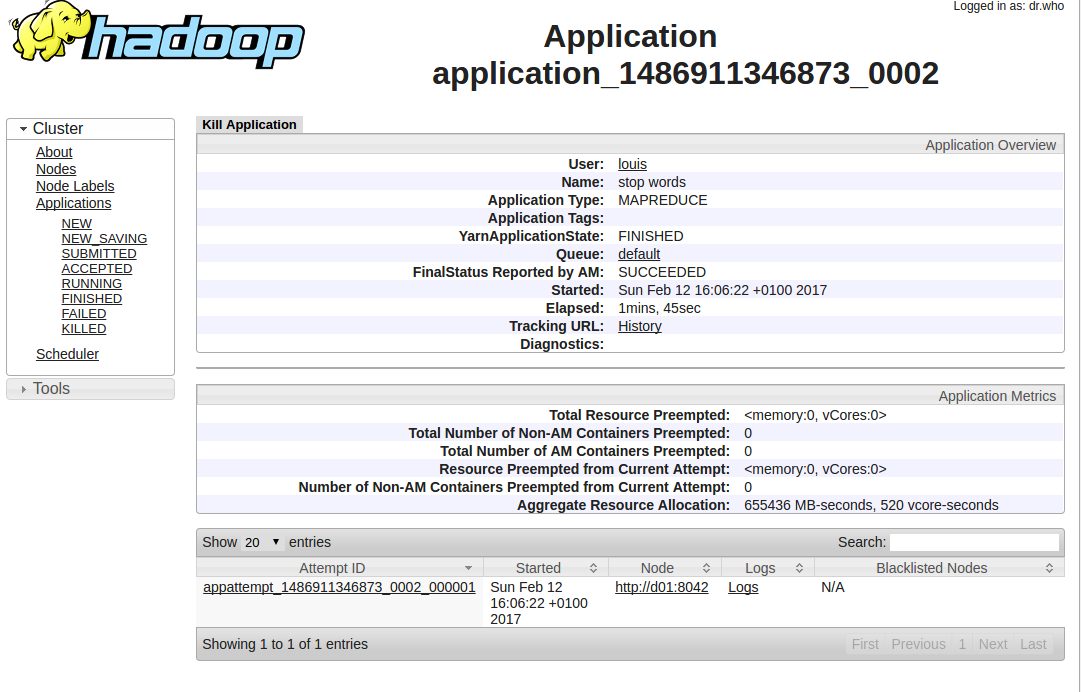
\includegraphics[width=.6\textwidth]{stopwords_10_reducers_1_combiner.png}
\end{figure}
\subsubsection{(5) 10 Reducers and Combiner and Compression}
Compression compresses the data between the mappers and the reducers.
The running time with 10 reducers, 1 combiner and compression is \textbf{125 seconds}.
The running time increased. This can be explained by the fact that compression adds
an additional overhead and its benefit is not used for a single node cluster!
Indeed compression is often use to reduce network transfer times, which does not
occur here as all the mappers and reducers are on the same device.
\begin{figure}[!htbp]
  \centering
  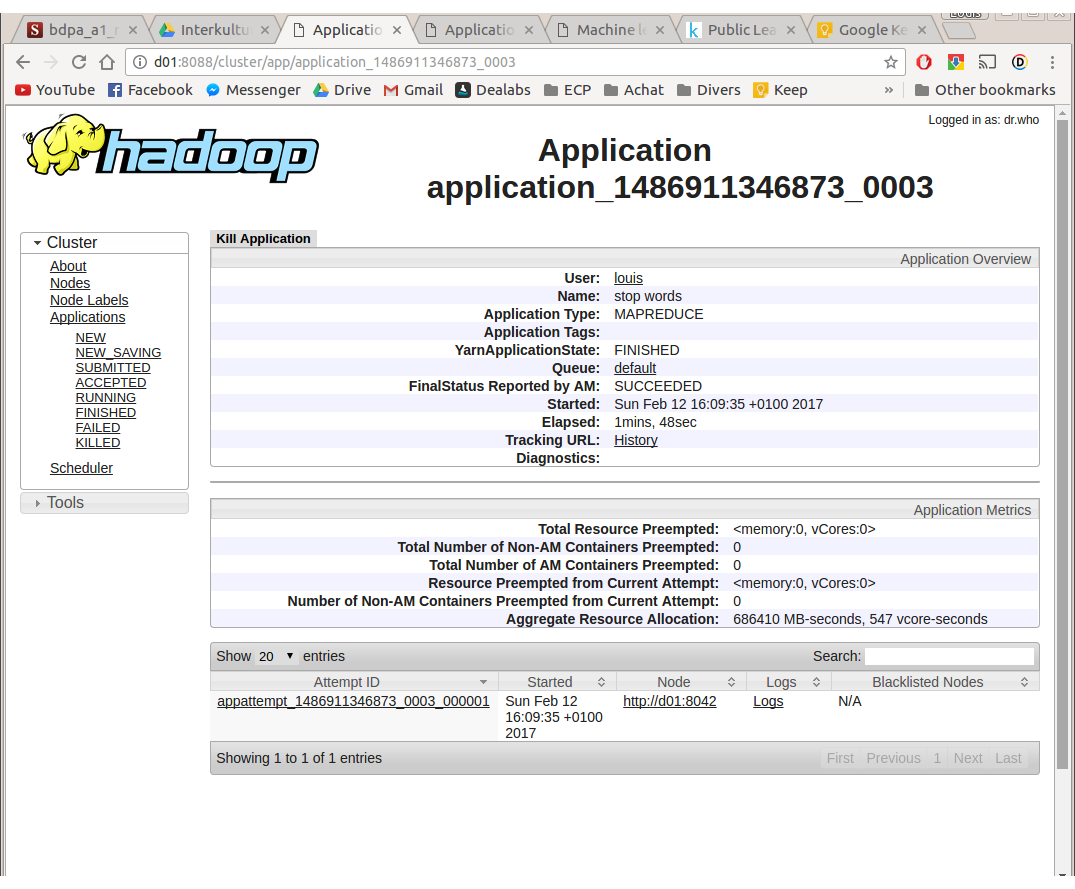
\includegraphics[width=.6\textwidth]{stopwords_10_reducers_1_combiner_compression.png}
\end{figure}

\subsubsection{(5) 50 Reducers and Combiner and Compression}
The running time with 50 reducers, 1 combiner and compression is \textbf{126 seconds}.
The running time is about the same as the previous experiment.
We did not benefit from the additional number of reducers.
This is logical because with a single node cluster, the processing power caps with
the limited number of cores. No additional gain is achieved with this extra parallelization.
\begin{figure}[!htbp]
  \centering
  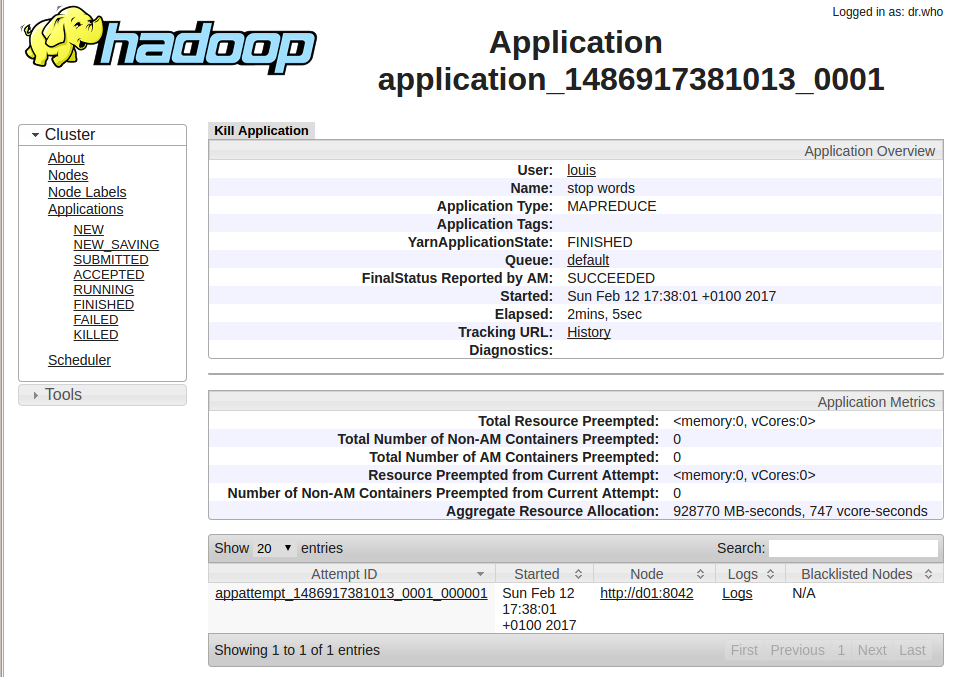
\includegraphics[width=.6\textwidth]{stopwords_50_reducers_1_combiner_compression.png}
\end{figure}

\subsection{(10) Unique words}
\begin{\begin{itemize}
  \item \textbf{readStopWords function:}\\
  First we need to read the stopwords from the csv file. We do it with the readStopWords function.
  This function is
  \lstinputlisting[firstnumber=30, firstline=30, lastline=62, language=java]{assets/InvertedIndex.java}
  \item \textbf{Mapper:}

\end{itemize}
\subsection{(30) Inverted index with frequency}

\section{(30) Bonus: Relative frequencies}

\end{document}

Dear all,

for the next assignments you are expected to provide on due date the your source code and a report of 10-20 pages.

Regarding the source code, it should be put on a Git repository, one per person. Please send to Pr. Christophides and me as soon as possible your URL to your Git repositories. You can either use github.com, bitbucket.org. If you intend to use GitLab, please consider using Central's GitLab in priority (https://gitlab.my.ecp.fr/users/sign_in). Whatever the Git repo, we must have access to your commit tree.

Regarding the report, here are some indication about what we would expect:

 1 - a quick walkthrough on your Hadoop setup (use hadoop version|checknative -a|dfsadmin) with the virtual machine specs (#core, #ram, HDD ...). Explain why you changed the defaults.

 2 - explanations on your implementations in particular the mapper/reducer codes and any data types extension you may make

 3 - an explanation on the data set including any assumptions or simplifications you made  to generate/process the data

 4 - the test scenario and the results for each one of them (including screenshots of the resource manager and the job tracker proving your run times)

 5 - conclusion


If you have any questions, please feel free to ask me by email.
But please, be concise, include relevant screenshots and error messages.
And last but not least KISS, DRY and YAGNI.

Regards,
Julien
